%%%%%%%%%%%%%%%%%%%%%%%%%%%%%%%%%%%%

\section{Examining numerical data}

%%%%%%%%%%%%%%%%%%%%%%%%%%%%%%%%%%%%

\subsection{Scatterplots for paired data}

%%%%%%%%%%%%%%%%%%%%%%%%%%%%%%%%%%%%

\begin{frame}
\frametitle{Scatterplot}

\hl{Scatterplots} are useful for visualizing the relationship between two numerical variables.

\begin{columns}[c]

\column{0.6 \textwidth}

\dq{Do life expectancy and total fertility appear to be \hl{associated} or \hl{independent}?}

\soln{\onslide<2->{They appear to be linearly and negatively associated: as fertility increases, life expectancy decreases.}}

\dq{Was the relationship the same throughout the years, or did it change?}

\soln{\onslide<3->{The relationship changed over the years.}}

\column{0.4 \textwidth}

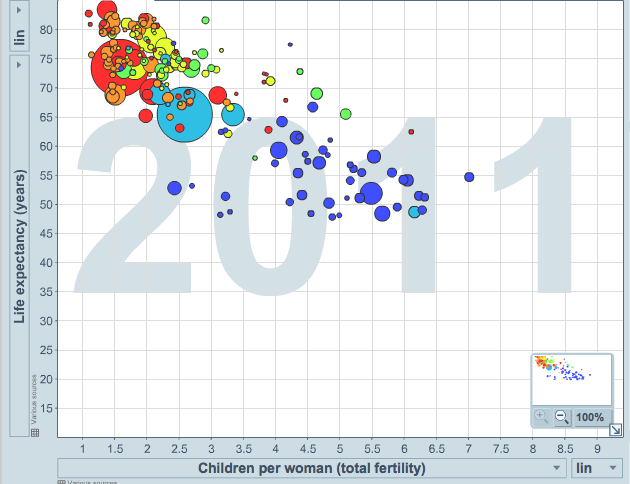
\includegraphics[width=\textwidth]{2-1_numerical_data/figures/life_exp_child}

\end{columns}

\ct{\webURL{http://www.gapminder.org/world}}

\end{frame}

%%%%%%%%%%%%%%%%%%%%%%%%%%%%%%%%%%%%

\subsection{Dot plots and the mean}

%%%%%%%%%%%%%%%%%%%%%%%%%%%%%%%%%%%%

\begin{frame}
\frametitle{Dot plots}

Useful for visualizing one numerical variable. Darker colors represent areas where there are more observations.

\begin{center}
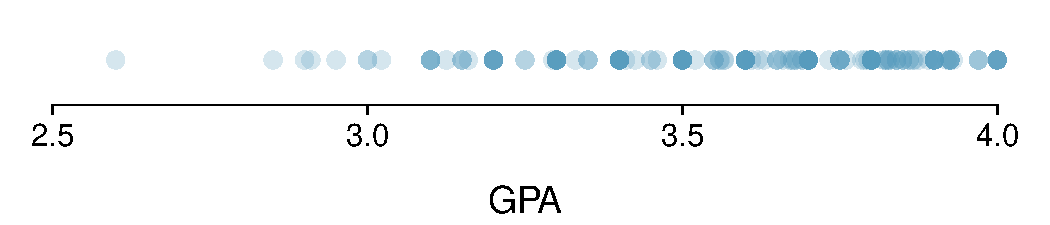
\includegraphics[width=\textwidth]{2-1_numerical_data/figures/gpa_dot_plot/gpa_dot_plot}
\end{center}

\dq{How would you describe the distribution of GPAs in this data set? Make sure to say something about the center, shape, and spread of the distribution.}

\end{frame}

%%%%%%%%%%%%%%%%%%%%%%%%%%%%%%%%%%%%


\begin{frame}
\frametitle{Dot plots \& mean}

\begin{center}
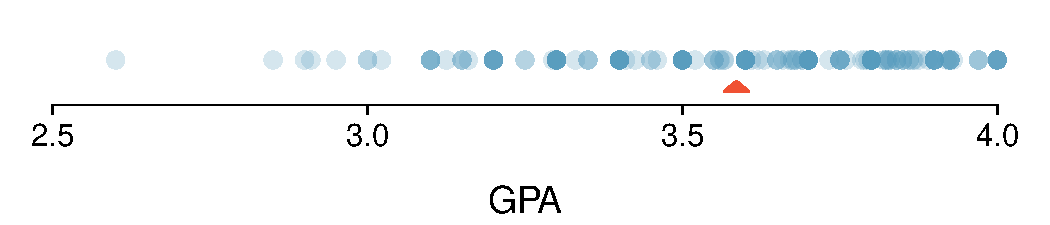
\includegraphics[width=\textwidth]{2-1_numerical_data/figures/gpa_dot_plot/gpa_dot_plot_mean}
\end{center}

\begin{itemize}

\item The \hl{mean}, also called the \hl{average} (marked with a triangle in the above plot), is one way to measure the center of a \hl{distribution} of data.

\item The mean GPA is 3.59.

\end{itemize} 

\end{frame}

%%%%%%%%%%%%%%%%%%%%%%%%%%%%%%%%%%%%

\begin{frame}
\frametitle{Mean}

\begin{itemize}

\item The \hl{sample mean}, denoted as \mathhl{\bar{x}}, can be calculated as

\[ \bar{x} = \frac{x_1 + x_2 + \cdots + x_n}{n}, \]

where $x_1, x_2, \cdots, x_n$ represent the \hl{n} observed values.

\item The \hl{population mean} is also computed the same way but is denoted as \mathhl{\mu}. It is often not possible to calculate $\mu$ since population data are rarely available.

\item The sample mean is a \hl{sample statistic}, and serves as a \hl{point estimate} of the population mean. This estimate may not be perfect, but if the sample is good (representative of the population), it is usually a pretty good estimate. 

\end{itemize}

\end{frame}

%%%%%%%%%%%%%%%%%%%%%%%%%%%%%%%%%%%%

\begin{frame}
\frametitle{Stacked dot plot}

Higher bars represent areas where there are more observations, makes it a little easier to judge the center and the shape of the distribution.

\begin{center}
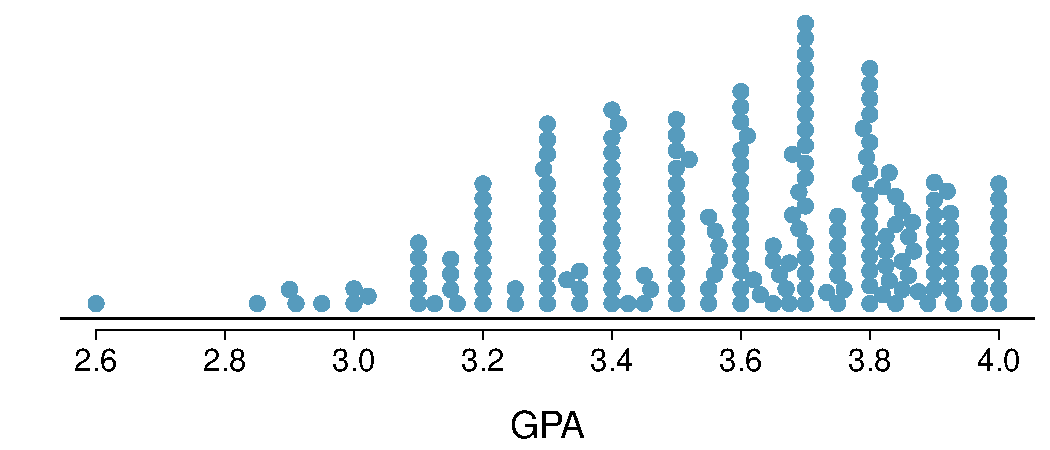
\includegraphics[width=\textwidth]{2-1_numerical_data/figures/gpa_dot_plot/gpa_dot_plot_stacked}
\end{center}

\end{frame}

%%%%%%%%%%%%%%%%%%%%%%%%%%%%%%%%%%%%

\subsection{Histograms and shape}

%%%%%%%%%%%%%%%%%%%%%%%%%%%%%%%%%%%%

\begin{frame}[fragile]
\frametitle{Histograms - Extracurricular hours}

\begin{itemize}

\item Histograms provide a view of the \hl{data density}. Higher bars represent where the data are relatively more common.

\item Histograms are especially convenient for describing the \hl{shape} of the data distribution.

\item The chosen \hl{bin width} can alter the story the histogram is telling.

\end{itemize}

\begin{center}
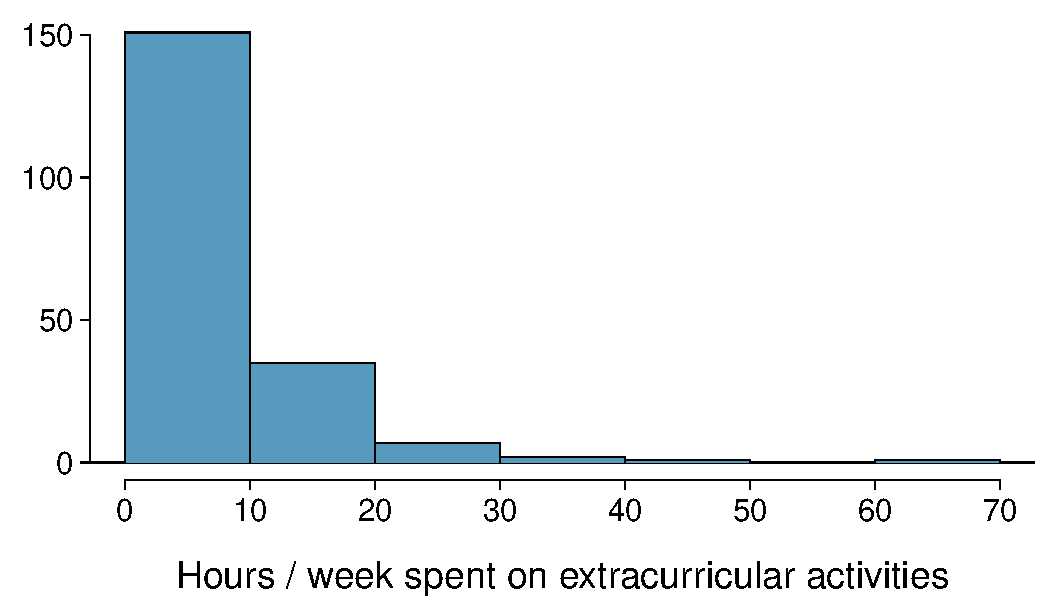
\includegraphics[width=0.75\textwidth]{2-1_numerical_data/figures/extracurr_hrs_hist/extracurr_hrs_hist}
\end{center}

\end{frame}

%%%%%%%%%%%%%%%%%%%%%%%%%%%%%%%%%%%%

\begin{frame}
\frametitle{Bin width}

\dq{Which one(s) of these histograms are useful? Which reveal too much about the data? Which hide too much?}

\begin{center}
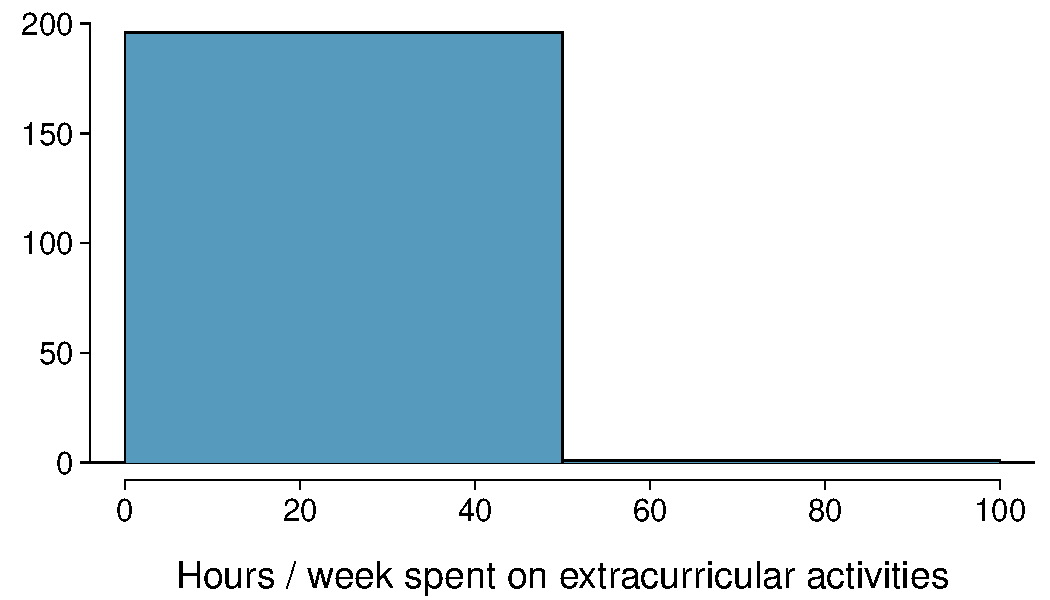
\includegraphics[width=0.45\textwidth]{2-1_numerical_data/figures/extracurr_hrs_hist/extracurr_hrs_hist2}
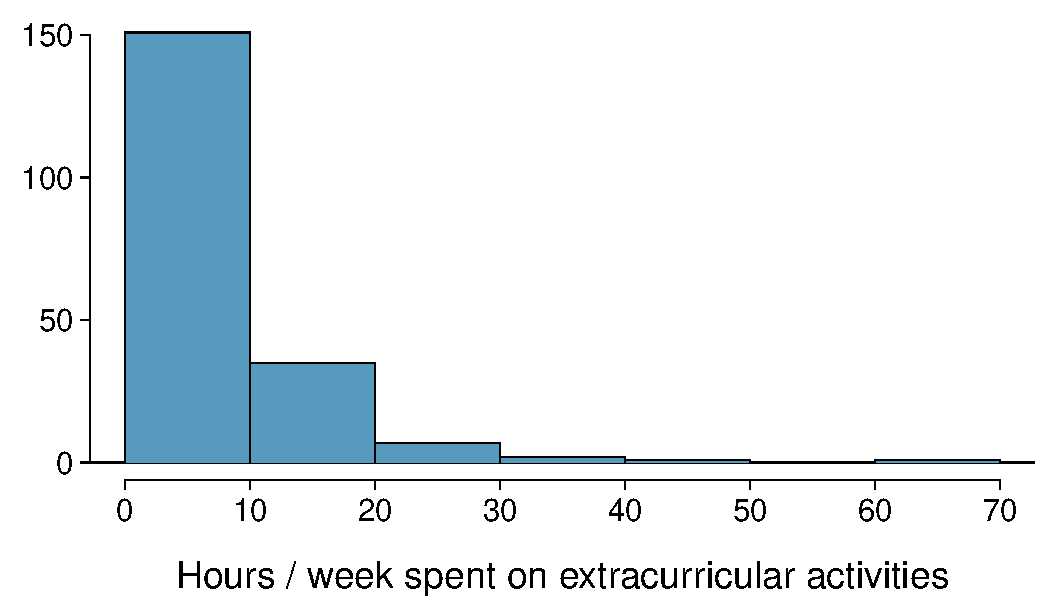
\includegraphics[width=0.45\textwidth]{2-1_numerical_data/figures/extracurr_hrs_hist/extracurr_hrs_hist} \\
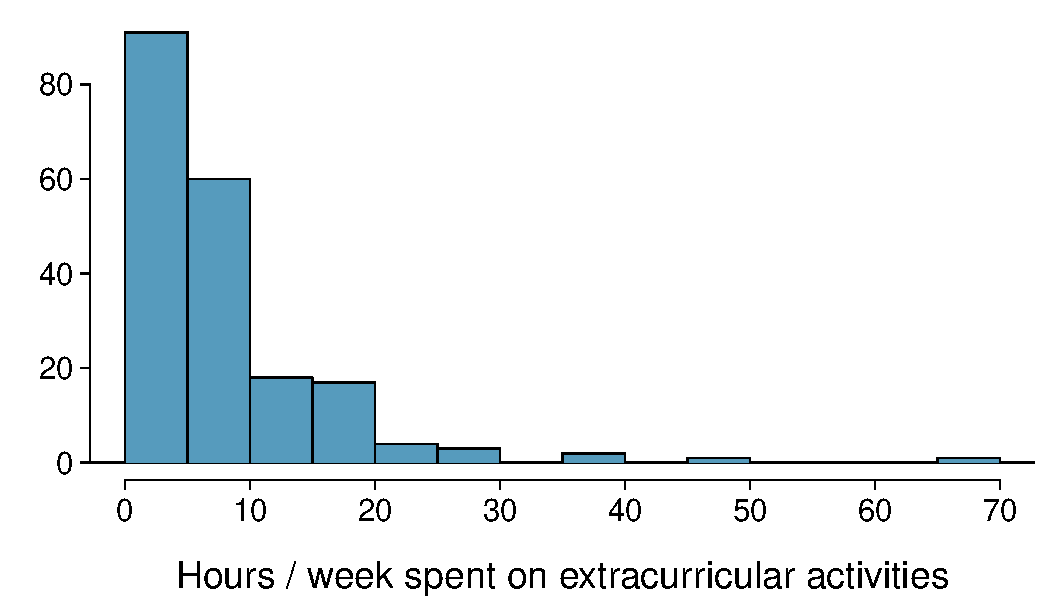
\includegraphics[width=0.45\textwidth]{2-1_numerical_data/figures/extracurr_hrs_hist/extracurr_hrs_hist20}
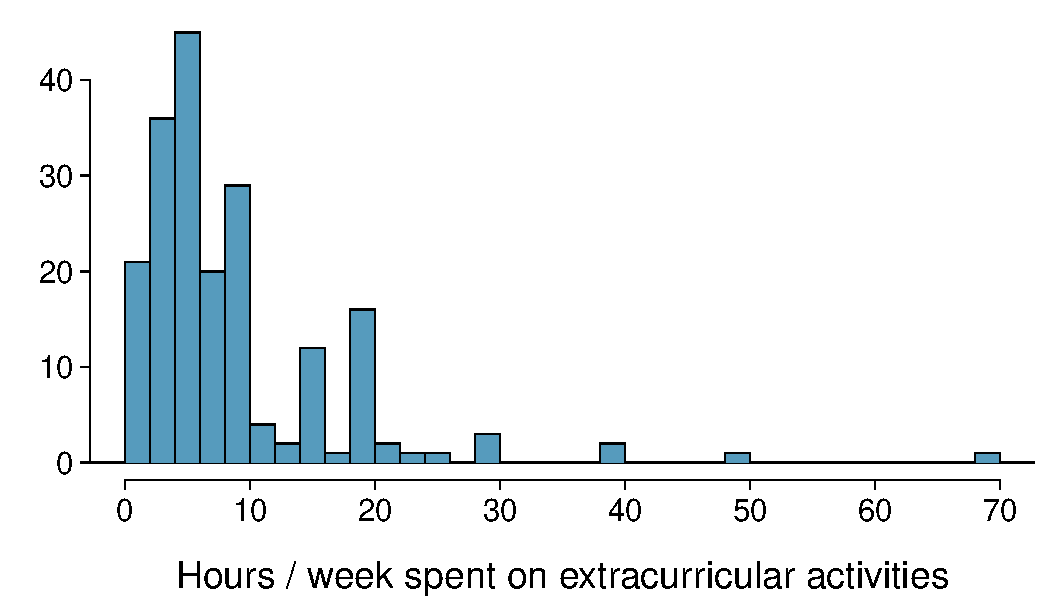
\includegraphics[width=0.45\textwidth]{2-1_numerical_data/figures/extracurr_hrs_hist/extracurr_hrs_hist30}
\end{center}

\end{frame}

%%%%%%%%%%%%%%%%%%%%%%%%%%%%%%%%%%%%

\begin{frame}
\frametitle{Shape of a distribution: modality}

Does the histogram have a single prominent peak (\hl{unimodal}), several prominent peaks (\hl{bimodal/multimodal}), or no apparent peaks (\hl{uniform})?

\begin{center}
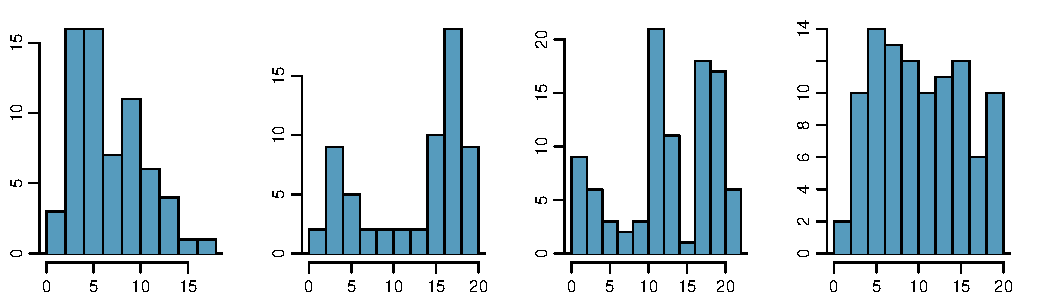
\includegraphics[width=0.75\textwidth]{2-1_numerical_data/figures/singleBiMultiModalUnifPlots/singleBiMultiModalUnifPlots}
\end{center}

\Note{In order to determine modality, step back and imagine a smooth curve over the histogram -- imagine that the bars are wooden blocks and you drop a limp spaghetti over them, the shape the spaghetti would take could be viewed as a smooth curve.}

\end{frame}

%%%%%%%%%%%%%%%%%%%%%%%%%%%%%%%%%%%%

\begin{frame}
\frametitle{Shape of a distribution: skewness}

Is the histogram \hl{right skewed}, \hl{left skewed}, or \hl{symmetric}?

\begin{center}
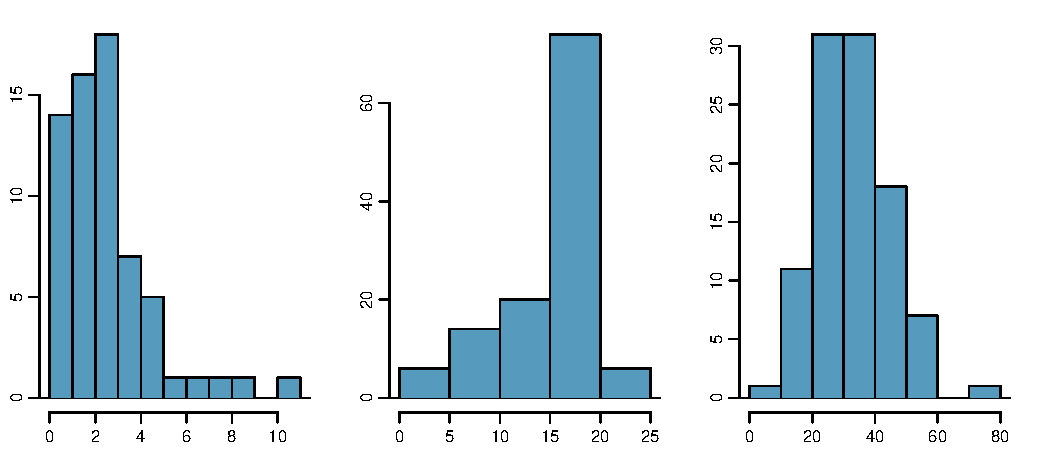
\includegraphics[width=0.8\textwidth]{2-1_numerical_data/figures/skewedSymPlots/skewedSymPlots}
\end{center}

\Note{Histograms are said to be skewed to the side of the long tail.}

\end{frame}

%%%%%%%%%%%%%%%%%%%%%%%%%%%%%%%%%%%%

\begin{frame}
\frametitle{Shape of a distribution: unusual observations}

Are there any unusual observations or potential \hl{outliers}?

\begin{center}
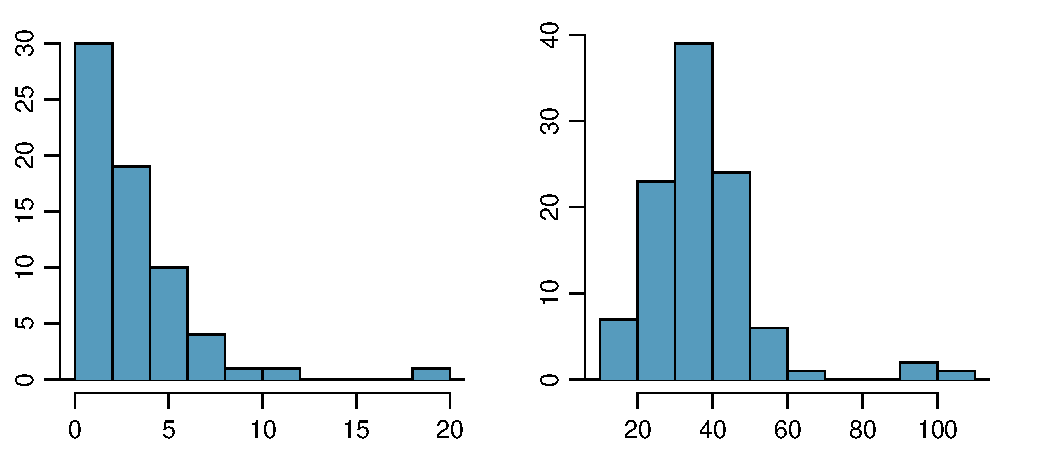
\includegraphics[width=0.8\textwidth]{2-1_numerical_data/figures/outlierPlots/outlierPlots}
\end{center}

\end{frame}

%%%%%%%%%%%%%%%%%%%%%%%%%%%%%%%%%%%%

\begin{frame}
\frametitle{Extracurricular activities}

\dq{How would you describe the shape of the distribution of hours per week students spend on extracurricular activities?}

\begin{center}
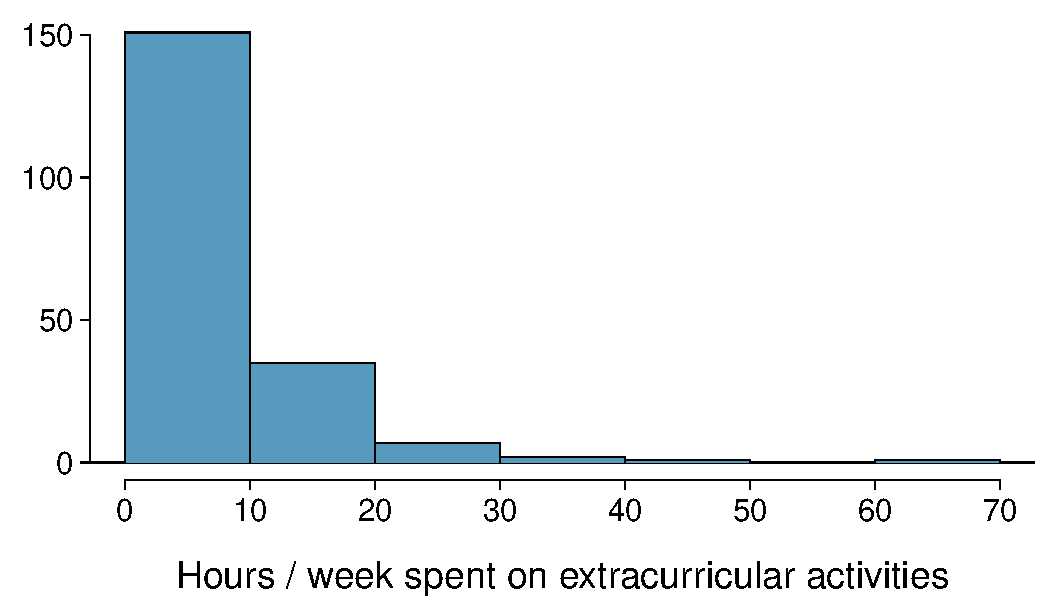
\includegraphics[width=0.75\textwidth]{2-1_numerical_data/figures/extracurr_hrs_hist/extracurr_hrs_hist}
\end{center}

\soln{\pause{Unimodal and right skewed, with a potentially unusual observation at 60 hours/week.}}

\end{frame}

%%%%%%%%%%%%%%%%%%%%%%%%%%%%%%%%%%%%

\begin{frame}
\frametitle{Commonly observed shapes of distributions}

\begin{itemize}

\item modality \\
$\:$ \\
\pause

\begin{columns}[c]
\column{0.25\textwidth}
unimodal \\
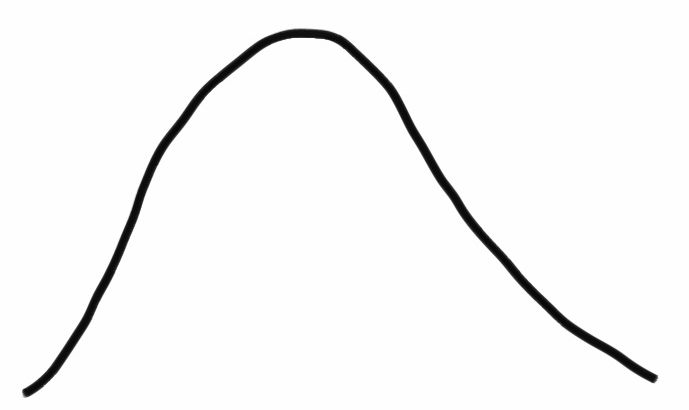
\includegraphics[width=\textwidth]{2-1_numerical_data/figures/shape_sketches/unimodal} 
\pause
\column{0.25\textwidth}
bimodal \\
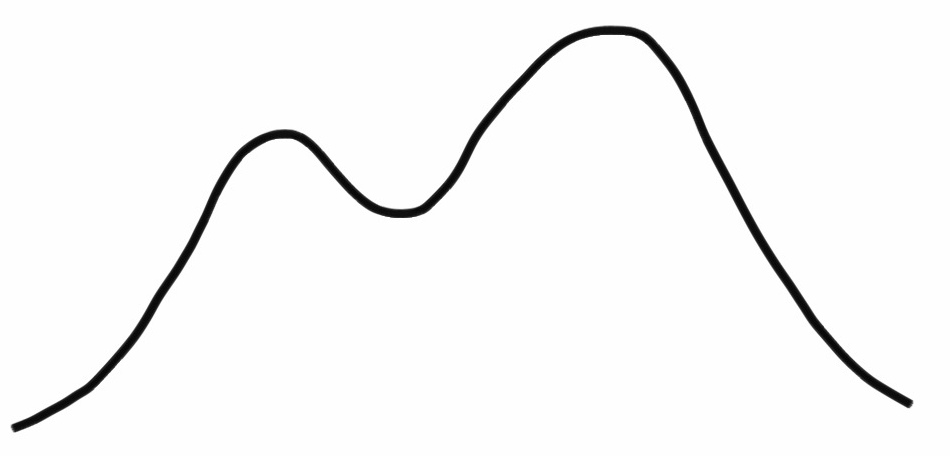
\includegraphics[width=\textwidth]{2-1_numerical_data/figures/shape_sketches/bimodal} 
\pause
\column{0.25\textwidth}
multimodal \\
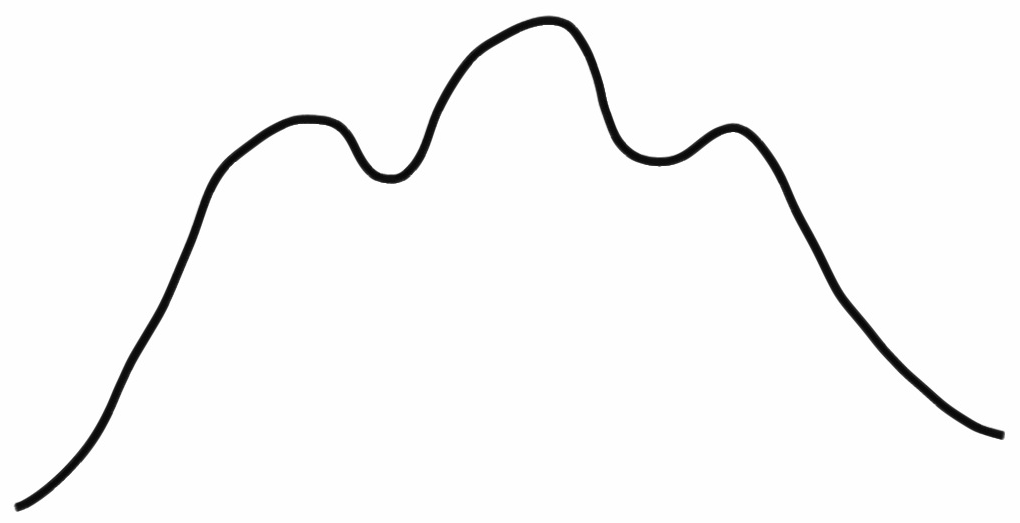
\includegraphics[width=\textwidth]{2-1_numerical_data/figures/shape_sketches/multimodal} 
\pause
\column{0.25\textwidth}
uniform
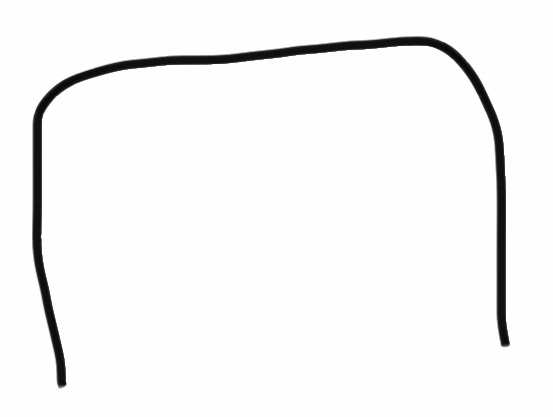
\includegraphics[width=\textwidth]{2-1_numerical_data/figures/shape_sketches/uniform} 
\end{columns}

\pause

$\:$ \\

\item skewness \\
$\:$ \\
\pause

\begin{columns}[c]
\column{0.25\textwidth}
right skew \\
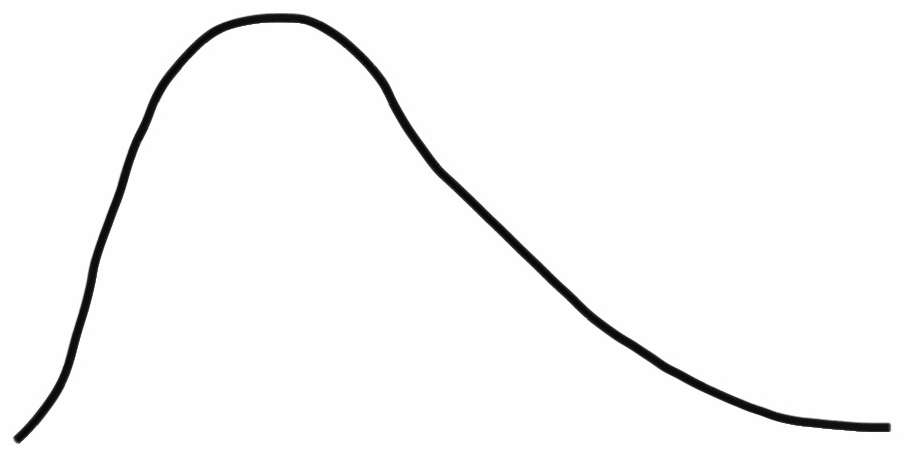
\includegraphics[width=\textwidth]{2-1_numerical_data/figures/shape_sketches/right_skew} 
\pause
\column{0.25\textwidth}
left skew \\
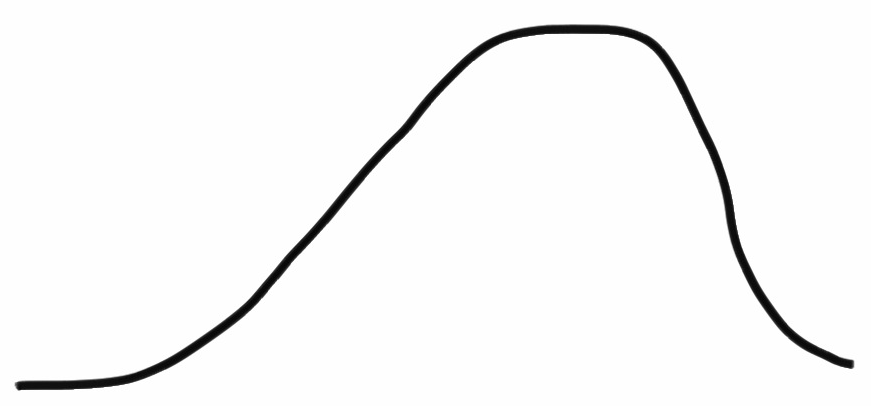
\includegraphics[width=\textwidth]{2-1_numerical_data/figures/shape_sketches/left_skew} 
\pause
\column{0.25\textwidth}
symmetric \\
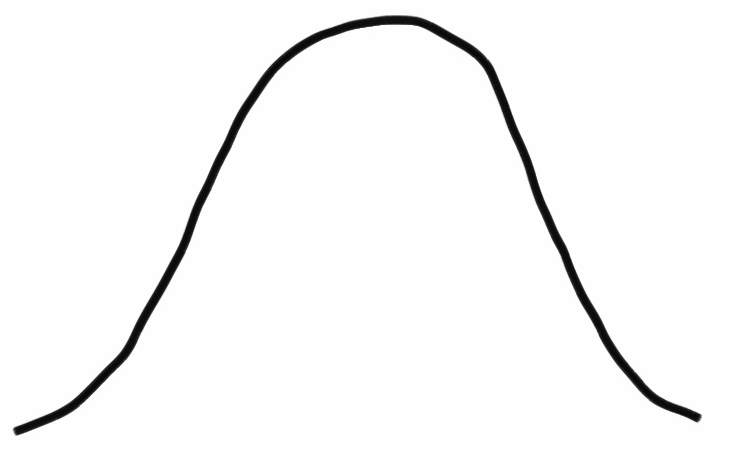
\includegraphics[width=\textwidth]{2-1_numerical_data/figures/shape_sketches/symmetric} 
\end{columns}

\end{itemize}

\end{frame}

%%%%%%%%%%%%%%%%%%%%%%%%%%%%%%%%%%%

\begin{frame}
\frametitle{Practice}

\pq{Which of these variables do you expect to be uniformly distributed?}

\begin{enumerate}[(a)]
\item weights of adult females
\item salaries of a random sample of people from North Carolina
\item house prices
\solnMult{birthdays of classmates (day of the month)}
\end{enumerate}

\end{frame}

%%%%%%%%%%%%%%%%%%%%%%%%%%%%%%%%%%%

\begin{frame}
\frametitle{Application activity: Shapes of distributions}

\app{Sketch the expected distributions of the following variables:
\begin{itemize}
\item number of piercings
\item scores on an exam
\item IQ scores
\end{itemize}
Come up with a concise way (1-2 sentences) to teach someone how to determine the expected distribution of any variable.
}

\end{frame}

%%%%%%%%%%%%%%%%%%%%%%%%%%%%%%%%%%%

\begin{frame}
\frametitle{Are you typical?}

\begin{center}
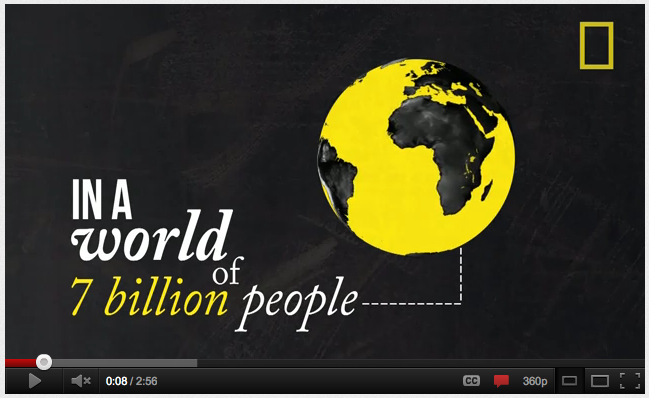
\includegraphics[width=0.75\textwidth]{2-1_numerical_data/figures/typical}
\end{center}

\begin{center}
\footnotesize{\webURL{http://www.youtube.com/watch?v=4B2xOvKFFz4}}
\end{center}

\pause

\dq{How useful are centers alone for conveying the true characteristics of a distribution?}

\end{frame}

%%%%%%%%%%%%%%%%%%%%%%%%%%%%%%%%%%%%

\subsection{Variance and standard deviation}

%%%%%%%%%%%%%%%%%%%%%%%%%%%%%%%%%%%

\begin{frame}
\frametitle{Variance}

\hl{Variance} is roughly the average squared deviation from the mean.

\formula{
\[ s^2 = \frac{\sum_{i = 1}^n (x_i - \bar{x})^2}{n - 1} \]
}

\pause

\twocol{0.5}{0.5}
{
\begin{itemize}

\item The sample mean is $\bar{x} = 6.71$, and the sample size is $n = 217$.

\onslide<3->{\item The variance of amount of sleep students get per night can be calculated as:}
\end{itemize}
}
{
\onslide<2->{
\begin{center}
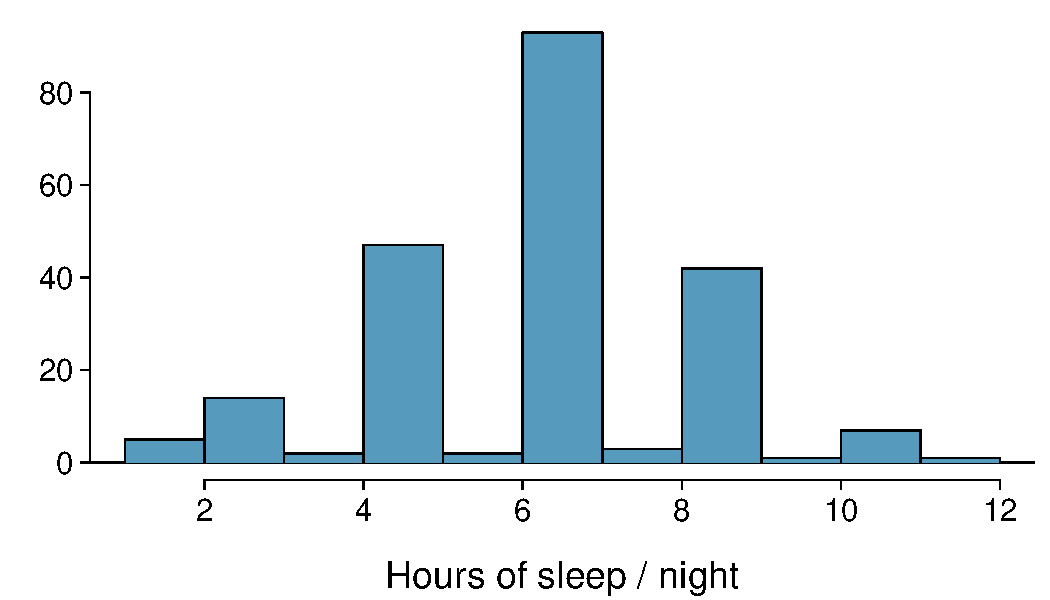
\includegraphics[width=\textwidth]{2-1_numerical_data/figures/sleep_hist/sleep_hist}
\end{center}
}
}
$\:$
\onslide<3->{
\[ s^2 = \frac{(5 - 6.71)^2 + (9 - 6.71)^2 + \cdots + (7 - 6.71)^2}{217 - 1} = 4.11~hours^2 \]
}



\end{frame}

%%%%%%%%%%%%%%%%%%%%%%%%%%%%%%%%%%%

\begin{frame}
\frametitle{Variance (cont.)}

\dq{Why do we use the squared deviation in the calculation of variance?}

\soln{\pause
\begin{itemize}
\item To get rid of negatives so that observations equally distant from the mean are weighed equally.
\item To weigh larger deviations more heavily.
\end{itemize}
}

\end{frame}

%%%%%%%%%%%%%%%%%%%%%%%%%%%%%%%%%%

\begin{frame}
\frametitle{Standard deviation}

The \hl{standard deviation} is the square root of the variance, and has the same units as the data.s

\formula{
\[ s = \sqrt{s^2} \]
}

\pause

\twocol{0.5}{0.5}
{
\begin{itemize}

\item The standard deviation of amount of sleep students get per night can be calculated as:
\[ s = \sqrt{4.11} = 2.03~hours\]

\onslide<3->{\item We can see that all of the data are within 3 standard deviations of the mean.}
\end{itemize}
}
{
\onslide<2->{
\begin{center}
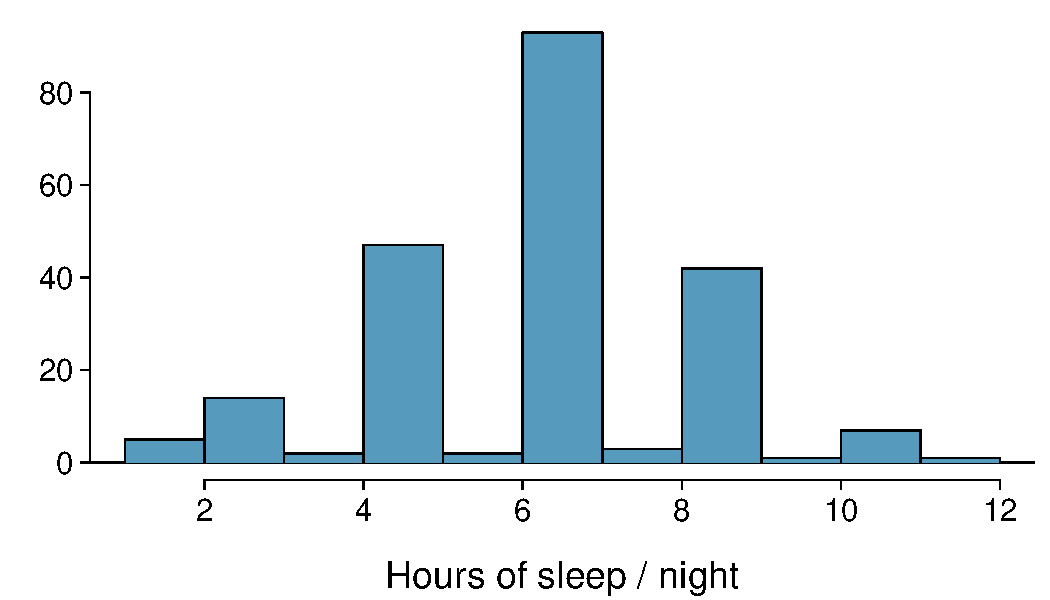
\includegraphics[width=\textwidth]{2-1_numerical_data/figures/sleep_hist/sleep_hist}
\end{center}
}
}

\end{frame}

%%%%%%%%%%%%%%%%%%%%%%%%%%%%%%%%%%%%

\subsection{Box plots, quartiles, and the median}

%%%%%%%%%%%%%%%%%%%%%%%%%%%%%%%%%%%%

\begin{frame}
\frametitle{Median}

\begin{itemize}

\item The \hl{median} is the value that splits the data in half when ordered in ascending order.

\[ 0,1,\orange{2},3,4 \]

\item If there are an even number of observations, then the median is the average of the two values in the middle.

\[ 0,1,\underline{2,3},4,5 \rightarrow \frac{2 + 3}{2} = \orange{2.5} \]

\item Since the median is the midpoint of the data, 50\% of the values are below it. Hence, it is also the \hl{$50^{th}$ percentile}.

\end{itemize}

\end{frame}

%%%%%%%%%%%%%%%%%%%%%%%%%%%%%%%%%%%%

\begin{frame}[fragile]
\frametitle{Q1, Q3, and IQR}

\begin{itemize}

\item The $25^{th}$ percentile is also called the first quartile, \hl{Q1}.

\item The $50^{th}$ percentile is also called the median.

\item The $75^{th}$ percentile is also called the third quartile, \hl{Q3}.

\item Between Q1 and Q3 is the middle 50\% of the data. The range these data span is called the \hl{interquartile range}, or the \hl{IQR}.
\formula{\[ IQR = Q3 - Q1 \]}
\end{itemize}

\end{frame}

%%%%%%%%%%%%%%%%%%%%%%%%%%%%%%%%%%%%

\begin{frame}
\frametitle{Box plot}

The box in a \hl{box plot} represents the middle 50\% of the data, and the thick line in the box is the median.

\begin{center}
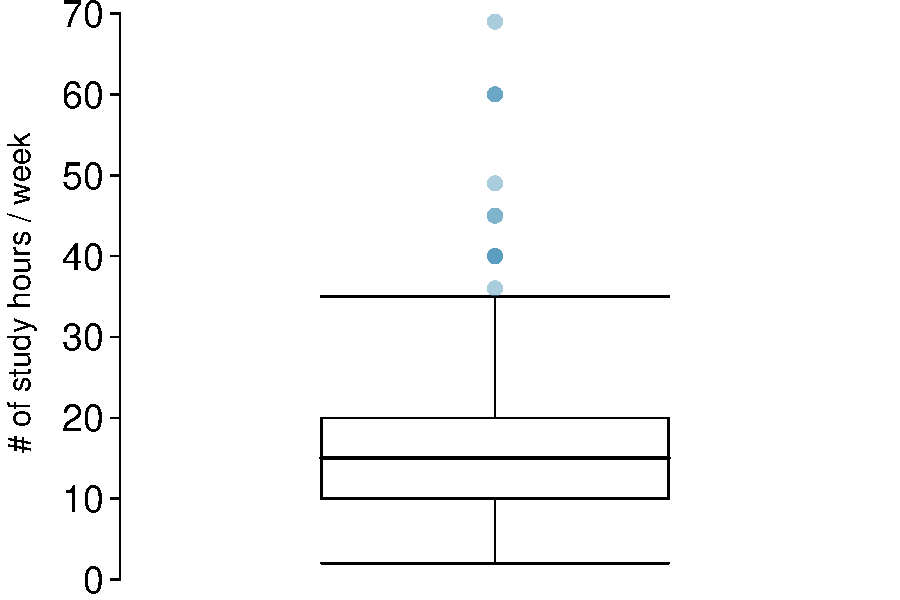
\includegraphics[width=0.7\textwidth]{2-1_numerical_data/figures/study_hours/study_hours_box}
\end{center}

\end{frame}

%%%%%%%%%%%%%%%%%%%%%%%%%%%%%%%%%%%%

\begin{frame}
\frametitle{Anatomy of a box plot}

\begin{center}
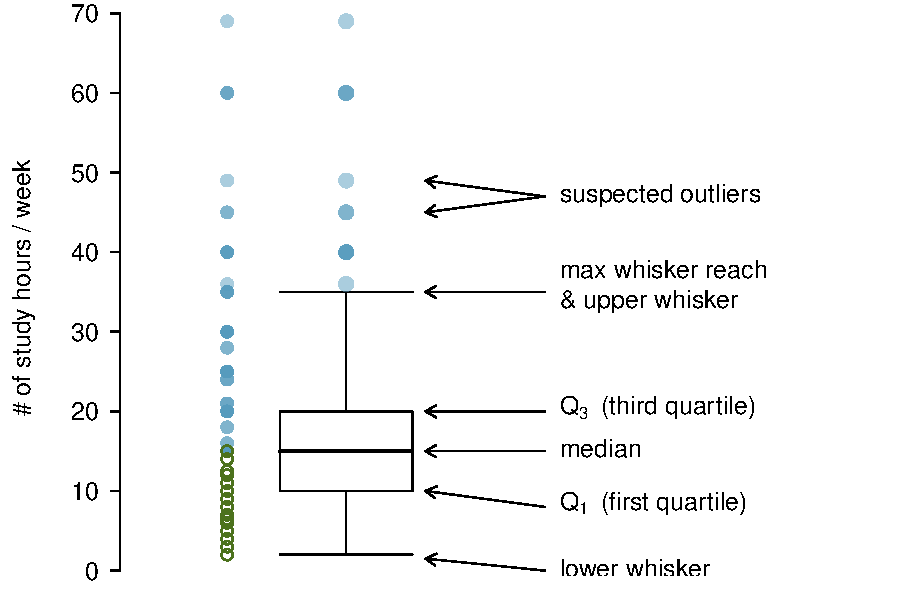
\includegraphics[width=0.95\textwidth]{2-1_numerical_data/figures/study_hours/study_hours_box_layout}
\end{center}

\end{frame}

%%%%%%%%%%%%%%%%%%%%%%%%%%%%%%%%%%%%

\begin{frame}[fragile]
\frametitle{Whiskers and outliers}

\begin{itemize}

\item \hl{Whiskers} of a box plot can extend up to $1.5 \times IQR$ away from the quartiles.
\formula{
\vspace{-0.5cm}
\begin{align*} 
\text{max~upper~whisker~reach} &= Q3 + 1.5 \times IQR \\
\text{max~lower~whisker~reach} &= Q1 - 1.5 \times IQR
\end{align*}
}
\pause
\vspace{-0.5cm}
{\small
\begin{align*}
\text{IQR}&: 20 - 10 = 10 \\
\text{max~upper~whisker~reach}&= 20 + 1.5 \times 10 = 35 \\
\text{max~lower~whisker~reach}&= 10 - 1.5 \times 10 = -5
\end{align*}
}

\pause
\vspace{-0.25cm}
\item A potential \hl{outlier} is defined as an observation beyond the maximum reach of the whiskers. It is an observation that appears extreme relative to the rest of the data.

\end{itemize}

\end{frame}

%%%%%%%%%%%%%%%%%%%%%%%%%%%%%%%%%%%%

\begin{frame}
\frametitle{Outliers (cont.)}

\dq{Why is it important to look for outliers?}

\soln{
\onslide<2->{
\begin{itemize}
\item Identify extreme skew in the distribution.
\item Identify data collection and entry errors.
\item Provide insight into interesting features of the data.
\end{itemize}
}
}

\end{frame}

%%%%%%%%%%%%%%%%%%%%%%%%%%%%%%%%%%%%

\subsection{Robust statistics}

%%%%%%%%%%%%%%%%%%%%%%%%%%%%%%%%%%%%

\begin{frame}
\frametitle{Extreme observations}

\dq{How would sample statistics such as mean, median, SD, and IQR of household income be affected if the largest value was replaced with \$10 million? What if the smallest value was replaced with \$10 million?}

\begin{center}
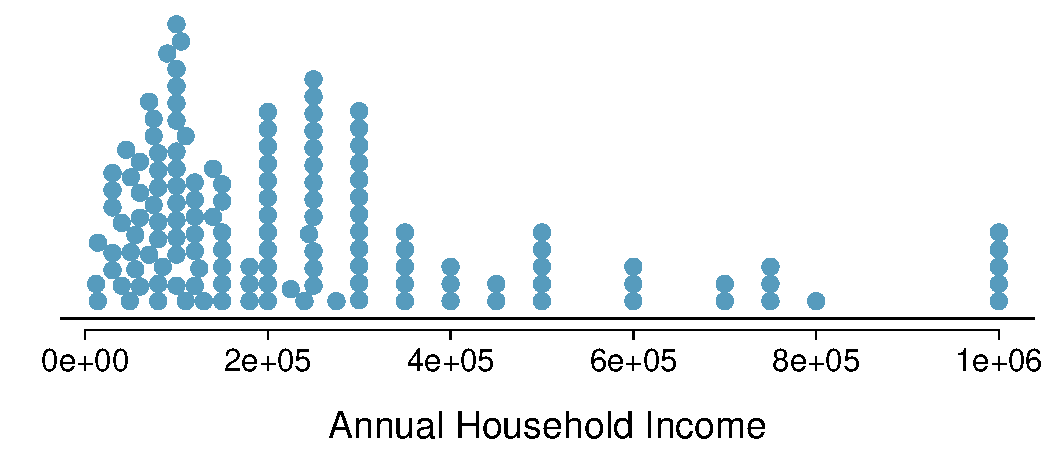
\includegraphics[width=\textwidth]{2-1_numerical_data/figures/house_income/house_income_dot_stacked}
\end{center}

\end{frame}

%%%%%%%%%%%%%%%%%%%%%%%%%%%%%%%%%%%%

\begin{frame}
\frametitle{Robust statistics}

\begin{center}
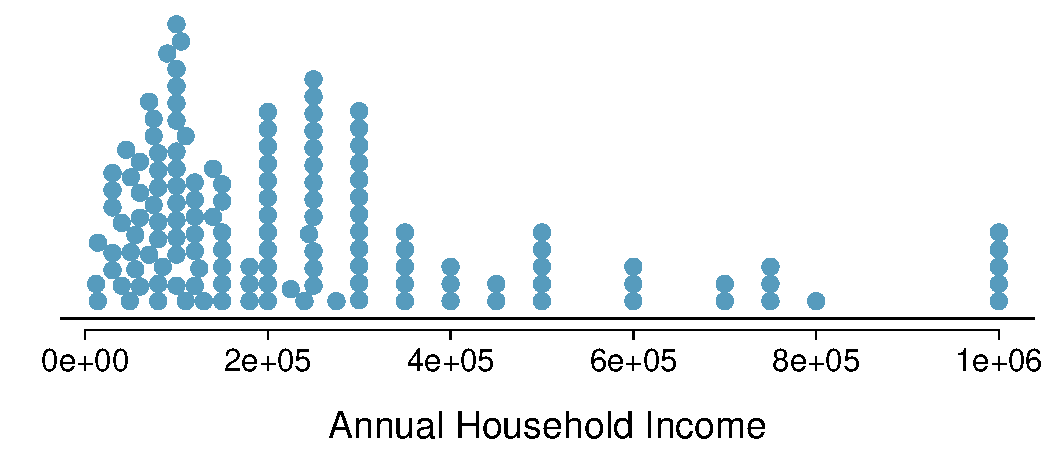
\includegraphics[width=\textwidth]{2-1_numerical_data/figures/house_income/house_income_dot_stacked}
\end{center}

{\small
\begin{center}
\begin{tabular}{l c cc c cc}
  \hline
& \hspace{0mm} & \multicolumn{2}{c}{\bf robust} & \hspace{2mm} & \multicolumn{2}{c}{\bf not robust} \\
scenario && median & IQR && $\bar{x}$ & $s$ \\ 
  \hline
original data && 190K & 200K && 245K & 226K \\ 
move largest to \$10 million && 190K & 200K && 309K & 853K \\ 
move smallest to \$10 million && 200K & 200K && 316K & 854K \\ 
   \hline
\end{tabular}
\end{center}
}

\end{frame}

%%%%%%%%%%%%%%%%%%%%%%%%%%%%%%%%%%%%

\begin{frame}
\frametitle{Robust statistics}

Median and IQR are more robust to skewness and outliers than mean and SD. Therefore,

\begin{itemize}
\item for skewed distributions it is often more helpful to use median and IQR to describe the center and spread
\item for symmetric distributions it is often more helpful to use the mean and SD to describe the center and spread
\end{itemize}

$\:$ \\

\pause

\dq{If you would like to estimate the typical household income for a student, would you be more interested in the mean or median income?}

\soln{\pause{Median}}

\end{frame}

%%%%%%%%%%%%%%%%%%%%%%%%%%%%%%%%%%%%

\begin{frame}
\frametitle{Mean vs. median}

\begin{itemize}

\item If the distribution is symmetric, center is often defined as the mean: mean $\approx$ median

\begin{center}
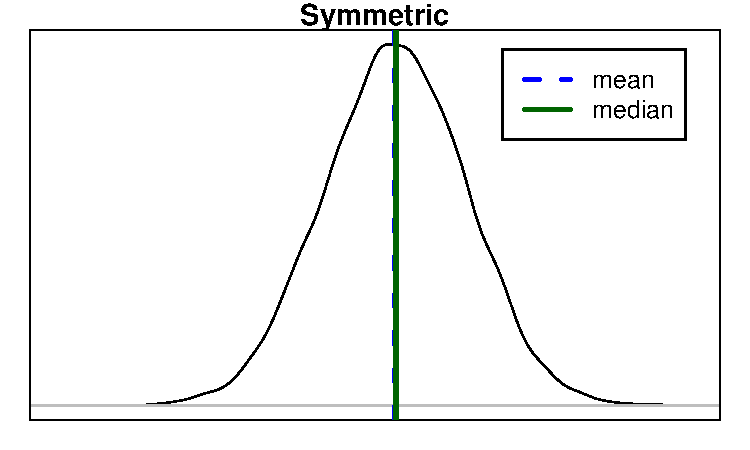
\includegraphics[width=0.33\textwidth]{2-1_numerical_data/figures/mean_med/sym}
\end{center}

\item If the distribution is skewed or has extreme outliers, center is often defined as the median
\begin{itemize}
\item Right-skewed: mean $>$ median
\item Left-skewed: mean $<$ median \\
\end{itemize}

\end{itemize}

\begin{center}
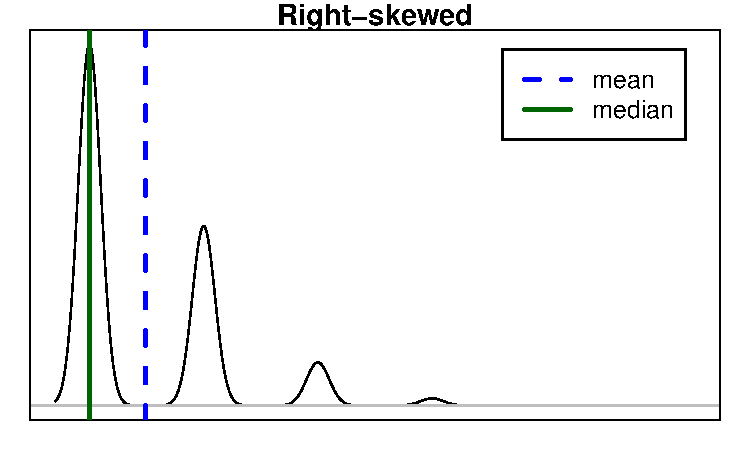
\includegraphics[width=0.33\textwidth]{2-1_numerical_data/figures/mean_med/rs}
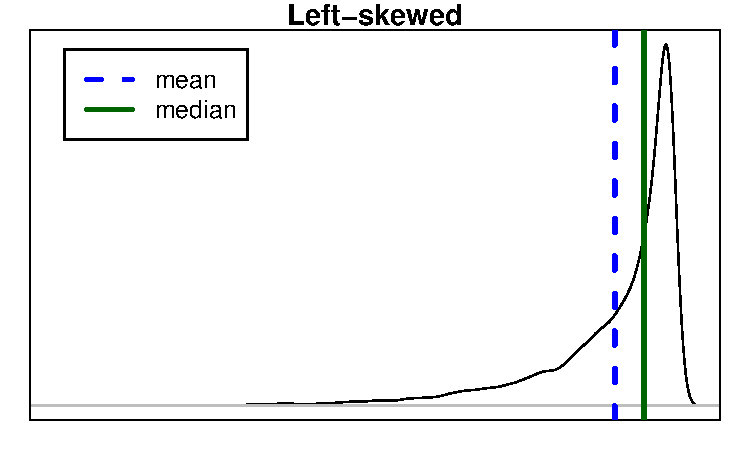
\includegraphics[width=0.33\textwidth]{2-1_numerical_data/figures/mean_med/ls}\\
\end{center}

\end{frame}

%%%%%%%%%%%%%%%%%%%%%%%%%%%%%%%%%%%%%

\begin{frame}
\frametitle{Practice}

\pq{{\small Which is most likely true for the distribution of percentage of time actually spent taking notes in class versus on Facebook, Twitter, etc.?}}

\vspace{-0.5cm}

\begin{columns}
\column{0.7\textwidth}
\begin{center}
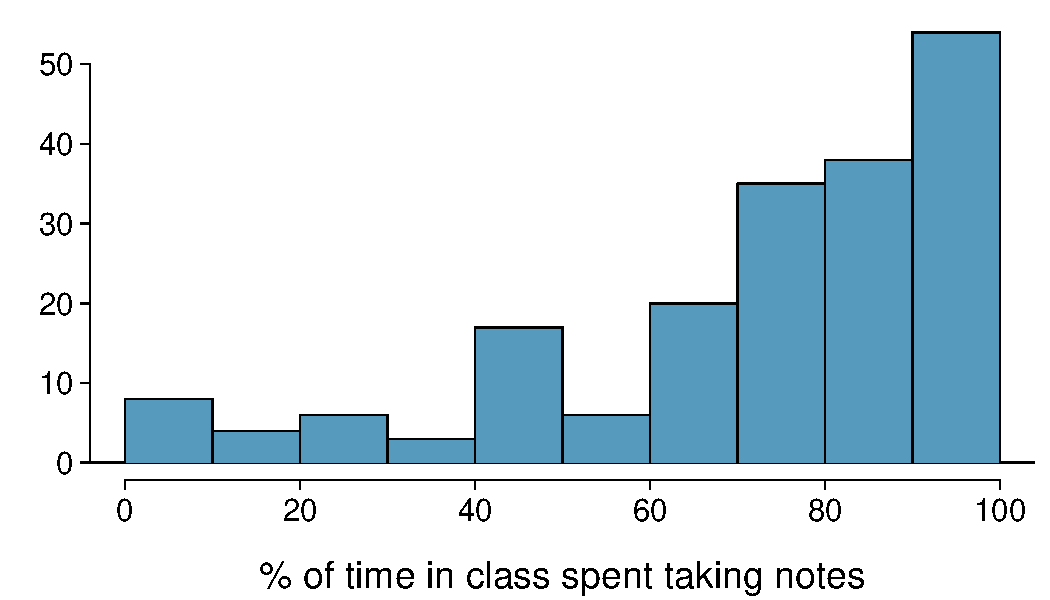
\includegraphics[width=0.9\textwidth]{2-1_numerical_data/figures/notes_perc/notes_perc_hist}
\end{center}
\column{0.3\textwidth}
$\:$ \\
$\:$ \\
\soln{\only<2>{\orange{median: 80\% \\ mean: 76\%}}}
\end{columns}

{\small
\begin{multicols}{2}
\begin{enumerate}[(a)]
\item mean$>$ median
\solnMult{mean $<$ median}
\item mean $\approx$ median
\item impossible to tell
\end{enumerate}
\end{multicols}
}

\end{frame}

%%%%%%%%%%%%%%%%%%%%%%%%%%%%%%%%%%%%%

\subsection{Transforming data}

%%%%%%%%%%%%%%%%%%%%%%%%%%%%%%%%%%%%

\begin{frame}
\frametitle{Extremely skewed data}

When data are extremely skewed, transforming them might make modeling easier. A common transformation is the \hl{log transformation}.

$\:$ \\
\pause
The histograms on the left shows the distribution of number of basketball games attended by students. The histogram on the right shows the distribution of log of number of games attended.

\begin{center}
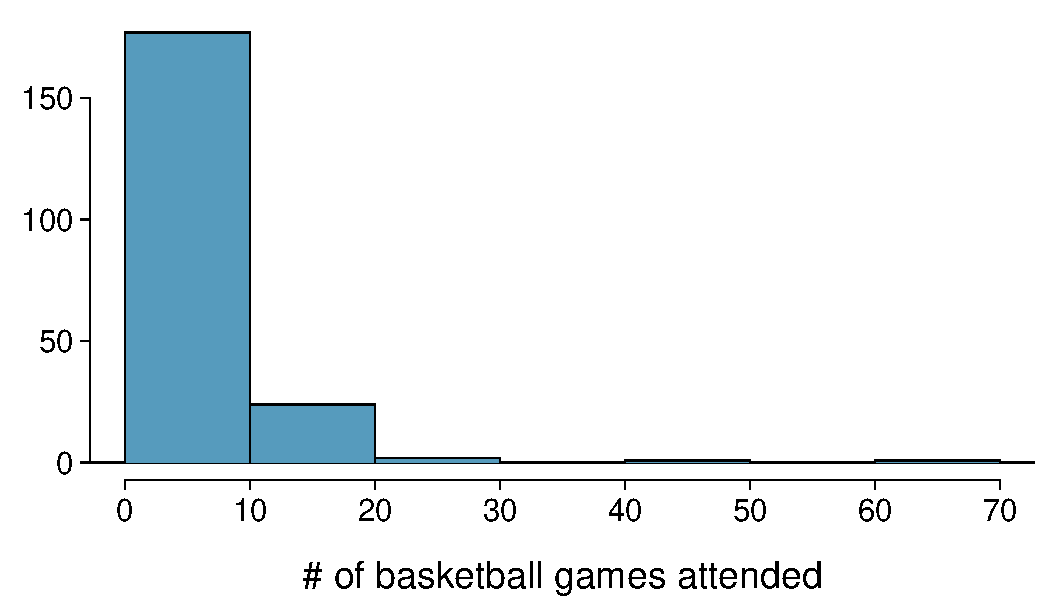
\includegraphics[width=0.5\textwidth]{2-1_numerical_data/figures/basket_games/basket_games_hist}
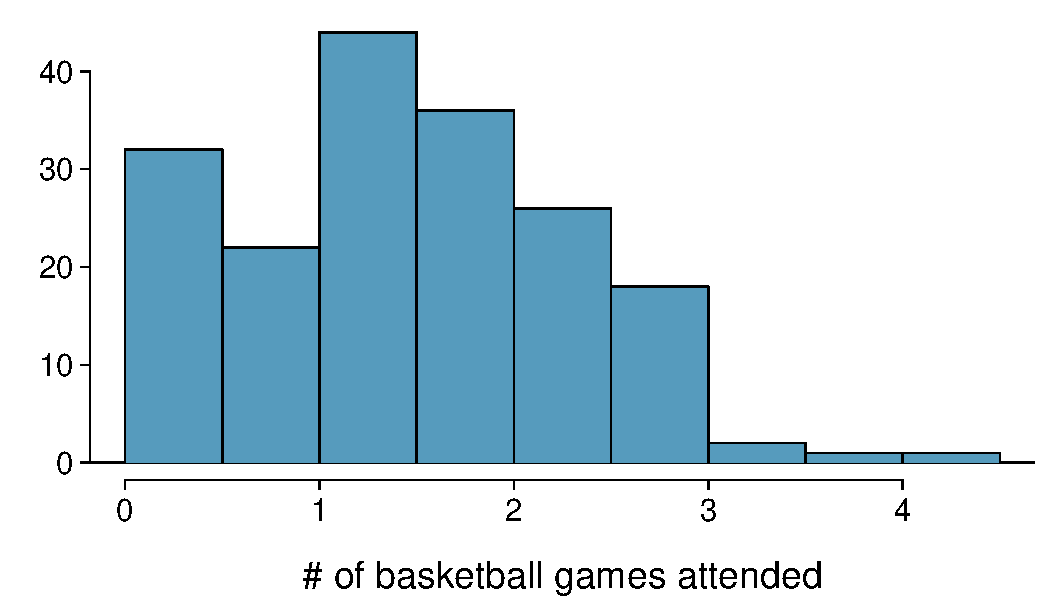
\includegraphics[width=0.5\textwidth]{2-1_numerical_data/figures/basket_games/basket_games_hist_log}
\end{center}

\end{frame}

%%%%%%%%%%%%%%%%%%%%%%%%%%%%%%%%%%%%

\begin{frame}
\frametitle{Pros and cons of transformations}

\begin{itemize}

\item Skewed data are easier to model with when they are transformed because outliers tend to become far less prominent after an appropriate transformation. \\
$\:$ \\
\renewcommand{\arraystretch}{1.5}
\begin{tabular}{l r r r r }
\# of games		&  70 	& 50 		& 25 		 		& $\cdots$ \\
log(\# of games)	& 4.25	& 3.91 	& 3.22 	 	& $\cdots$
\end{tabular}

$\:$ \\

\item However, results of an analysis in log units of the measured variable might be difficult to interpret.

\end{itemize}

\pause

\dq{What other variables would you expect to be extremely skewed?}

\soln{\pause{Salary, housing prices, etc.}}

\end{frame}

%%%%%%%%%%%%%%%%%%%%%%%%%%%%%%%%%%%%

\subsection{Mapping data}

%%%%%%%%%%%%%%%%%%%%%%%%%%%%%%%%%%%%

\begin{frame}
\frametitle{Intensity maps}

\dq{What patterns are apparent in the change in population between 2000 and 2010?}

\begin{center}
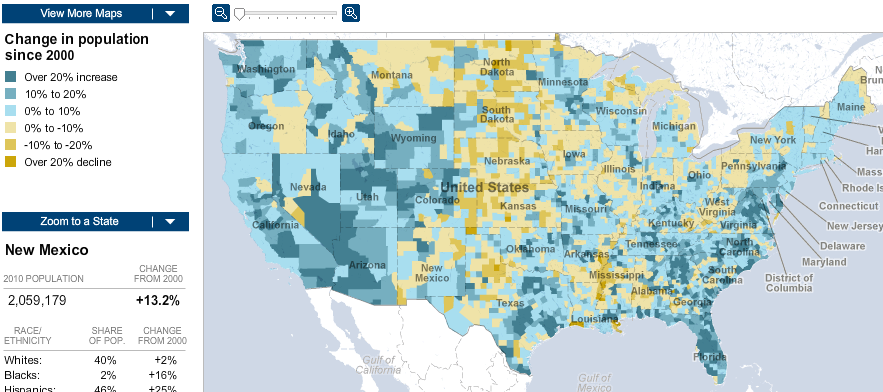
\includegraphics[width=0.95\textwidth]{2-1_numerical_data/figures/change_in_pop_intensity}
\end{center}

\ct{\webURL{http://projects.nytimes.com/census/2010/map}}

\end{frame}


%%%%%%%%%%%%%%%%%%%%%%%%%%%%%%%%%%%%